\documentclass[tikz,border=3.14mm]{standalone}
\usepackage{pgfplots}
\usetikzlibrary{intersections}
\pgfplotsset{compat=1.16}
\usetikzlibrary{math} % tikzmath, see p. 640 of the pgfmanual. 
\newcommand{\rr}{\mathbf{r}}
\newcommand{\cc}{\mathbf{c}}

\pgfdeclarelayer{background}
\pgfsetlayers{background,main}
\tikzset{
	expand bubble/.style={
		preaction={draw,line width=10.4pt, white},
		white,fill,draw,line width=10pt, gray!10
	},
}


\begin{document}
	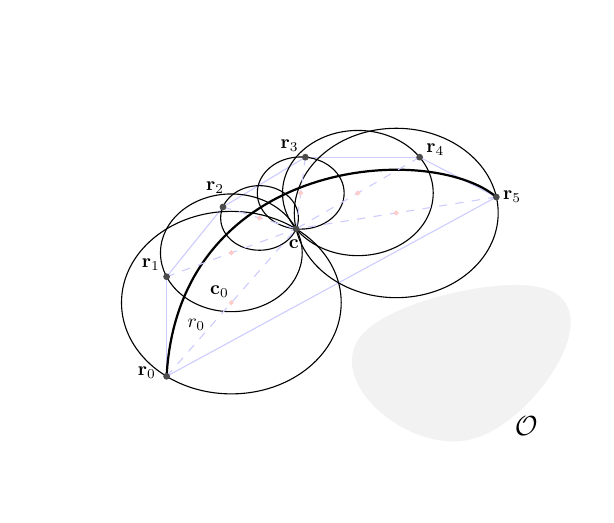
\begin{tikzpicture}
		\begin{axis}[
			xmin= -1.0, xmax=3.5,
			ymin= -1.0, ymax=3.5,
			samples=101,
			use fpu=false,mark=none,
			axis line style={draw=none},
			tick style={draw=none},
			yticklabels={,,},
			xticklabels={,,},
			domain=0:2] 
			\addplot[mark=*, mark size=1pt, color=black!70] coordinates {(2.75,1.8)} node[right, color=black, scale=0.7] {$\rr_{5}$};
			\addplot[mark=*, mark size=1pt, color=black!70] coordinates {(2.11,2.2)} node[xshift=2mm, yshift=1mm,, color=black, scale=0.7] {$\rr_{4}$};
			\addplot[mark=*, mark size=1pt, color=black!70] coordinates {(1.157,2.2)} node[xshift=-2mm, yshift=1.5mm,, color=black, scale=0.7] {$\rr_{3}$};
			\addplot[mark=*, mark size=1pt, color=black!70] coordinates {(0.47,1.7)} node[xshift=-1mm, yshift=2.5mm, color=black, scale=0.7] {$\rr_{2}$};
			\addplot[mark=*, mark size=1pt, color=black!70] coordinates {(0,1)} node[xshift=-2mm, yshift=1.5mm,, color=black, scale=0.7] {$\rr_{1}$};
			\addplot[mark=*, mark size=1pt, color=black!70] coordinates {(0,0)} node[xshift=-2.5mm, yshift=0.5mm,, color=black, scale=0.7] {$\rr_{0}$};
			
			\addplot[mark=none, color=blue!20] coordinates {(2.11,2.2) (2.75,1.8)};
			\addplot[mark=none, color=blue!20] coordinates {(1.157,2.2) (2.11,2.2)};
			\addplot[mark=none, color=blue!20] coordinates {(0.47,1.7) (1.157,2.2)};
			\addplot[mark=none, color=blue!20] coordinates {(0,1) (0.47,1.7)};
			\addplot[mark=none, color=blue!20] coordinates {(0,0) (0,1)};
			\addplot[mark=none, color=blue!20] coordinates {(0,0) (2.75,1.8)};
			
			\draw[thick, name path=curve] (0,0) .. controls (0.1,2.2) and (2.2,2.36) .. (2.75,1.8);

			\addplot[mark=*, mark size=1pt, color=black!70] coordinates {(1.08,1.48)} node[xshift=-0.3mm, yshift=-2mm, color=black, scale=0.7] {$\mathbf{c}$};
			
			\draw[, name path=circ1] (1.915,1.64) circle (0.8502);
			\draw[, name path=circ2] (1.595,1.84) circle (0.6284);
			\draw[, name path=circ3] (1.1185,1.84) circle (0.3621);
			\draw[, name path=circ4] (0.775,1.59) circle (0.3242);
			\draw[, name path=circ5] (0.54,1.24) circle (0.5909);
			\draw[, name path=circ6] (0.54,0.74) circle (0.9161);
			
			\addplot[dashed, mark=none, color=blue!20] coordinates {(2.11,2.2) (1.08,1.48)}; %node[pos=0.5, above, color=black, scale=0.7] {$r_4$};
			\addplot[dashed, mark=none, color=blue!20] coordinates {(1.157,2.2) (1.08,1.48)}; %node[pos=0.5, above, color=black, scale=0.7] {$r_3$};
			\addplot[dashed, mark=none, color=blue!20] coordinates {(0.47,1.7) (1.08,1.48)}; %node[pos=0.5, above, color=black, scale=0.7] {$r_2$};
			\addplot[dashed, mark=none, color=blue!20] coordinates {(0,1) (1.08,1.48)}; %node[pos=0.25, above, color=black, scale=0.7] {$r_1$};
			\addplot[dashed, mark=none, color=blue!20] coordinates {(0,0) (1.08,1.48)} node[pos=0.35, left, color=black, scale=0.7] {$r_0$};
			\addplot[dashed, mark=none, color=blue!20] coordinates {(2.75,1.8) (1.08,1.48)}; %node[pos=0.5, left, color=black, scale=0.7] {$r_5$};

			\addplot[mark=*, mark size=0.7pt, color=red!20] coordinates {(1.915,1.64)}; %node[right, color=black, scale=0.7] {$\cc_{5}$};
			\addplot[mark=*, mark size=0.7pt, color=red!20] coordinates {(1.595,1.84)}; %node[xshift=2mm, yshift=1mm,, color=black, scale=0.7] {$\cc_{4}$};
			\addplot[mark=*, mark size=0.7pt, color=red!20] coordinates {(1.1185,1.84)}; %node[xshift=1mm, yshift=1.5mm,, color=black, scale=0.7] {$\cc_{3}$};
			\addplot[mark=*, mark size=0.7pt, color=red!20] coordinates {(0.775,1.59)}; %node[above, color=black, scale=0.7] {$\cc_{2}$};
			\addplot[mark=*, mark size=0.7pt, color=red!20] coordinates {(0.54,1.24)}; %node[xshift=0.2mm, yshift=-1.2mm,, color=black, scale=0.7] {$\cc_{1}$};
			\addplot[mark=*, mark size=0.7pt, color=red!20] coordinates {(0.54,0.74)} node[xshift=-1.5mm, yshift=1.4mm,, color=black, scale=0.7] {$\cc_{0}$};

			%\draw[name path=circ5] (1.08,1.48) circle (1.8);
			
			\node (p1) at (1.7, 0.3) {};
			\node (p2) at (2.5, -0.5) {};
			\node (p3) at (3.2, 0.7) {};
			\node (p4) at (3.0, -0.5) {$\mathcal{O}$};
			\begin{pgfonlayer}{background}
				\path[expand bubble]plot [smooth cycle,tension=1] coordinates {(p1) (p2) (p3)};
			\end{pgfonlayer}
			
		\end{axis}
	\end{tikzpicture}
\end{document}